\chapter{}

\section{}
Das Nennmoment lässt sich anhand (\ref{eq:6:MN}) berechnen. Dabei lassen sich die benötigten Parameter vom Typenschild ablesen, wobei die Nenndrehzahl in $ s^{-1} $ umgerechnet werden muss.
\begin{equation}
	M_{N} = \frac{P_{N}}{2\pi N_{N}} = \frac{550W}{2\pi*3000min^{-1}} = \frac{550W}{2\pi*50s^{-1}} = 1.75Nm
	\label{eq:6:MN}
\end{equation}
Der Wirkungsgrad im Nennpunkt lässt sich wie in (\ref{eq:6:eta}) durch die zu- und abgeführte Leistung berechnen. Die abgeführte Leistung lässt sich direkt vom Typenschild ablesen, die zugeführte Leistung ergibt sich aus dem Produkt von Ankerspannung und -strom.
\begin{equation}
	\eta_{N} = \frac{P_{ab}}{P_{zu}} = \frac{P_{ab}}{U_{A}I_{A}} = \frac{550W}{180V*4.5A} = 67.9\%
	\label{eq:6:eta}
\end{equation}

\begin{figure}[h]
	\centering
	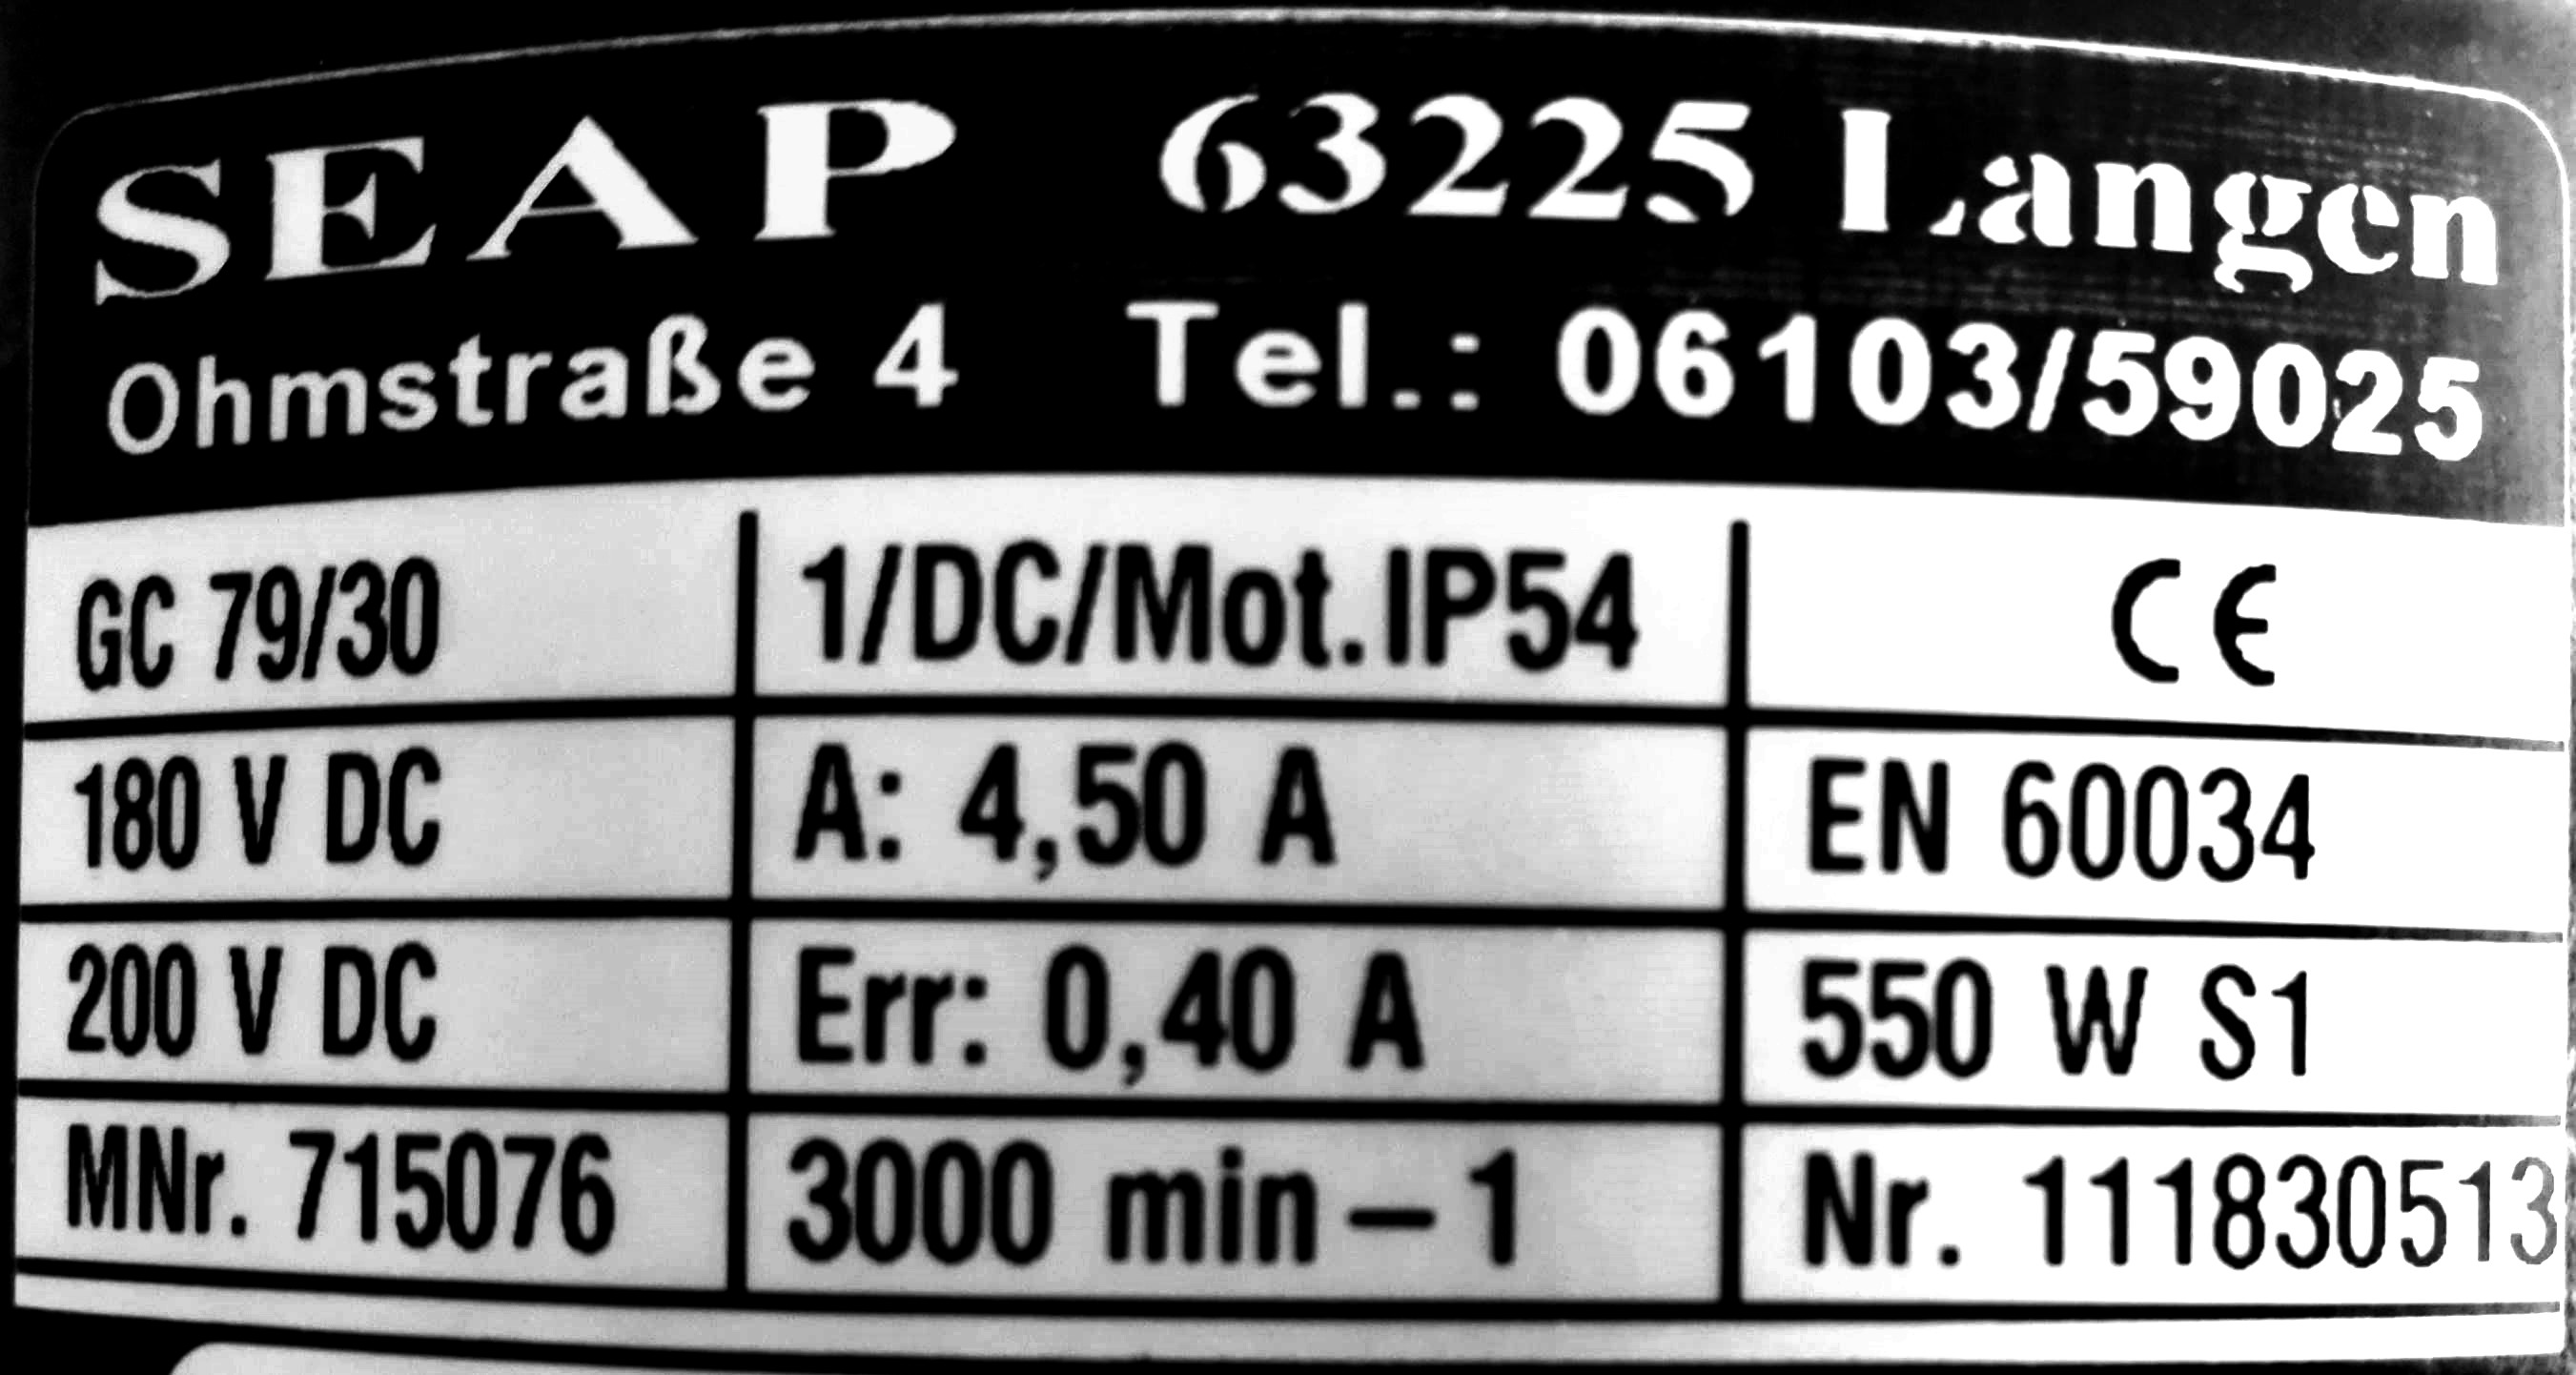
\includegraphics[width=0.8\textwidth]{./bilder/typenschild.jpg}
	\caption{Typenschild}
	\label{fig:typenschild}
\end{figure}